% Docummentation:
% - https://www.latex-project.org/help/documentation/
% - https://docs.w3cub.com/latex/
% - https://tex.stackexchange.com/questions/455993/formatting-sql-code
% - https://www.overleaf.com/learn/latex/Code_listing#Code_styles_and_colours

%--------------------------------------------------------------------------------
%-----------------------------------   TODO   ----------------------------------
%--------------------------------------------------------------------------------
% add section about icon source https://www.iconpacks.net/free-icon/money-bag-6384.html


\documentclass[a4paper,10pt, twoside]{report}

\usepackage{polski}         % Polish diacretic signs
\usepackage[utf8]{inputenc} % required for international characters
\usepackage{hyperref}       % urls and hyperlinks
\usepackage{xurl}           % break urls
\usepackage{microtype}      % improve justification
\usepackage{enumitem}       % compact lists
\usepackage{graphicx}       % Include graphics
\usepackage{wrapfig}        % wrap text aroung graphics
\usepackage{fancyhdr}       % Customize page layout
\usepackage{index}          % Create an index
\usepackage{setspace}       % Spacing
\usepackage{float}          % Forcing figure placement
\usepackage{tabularray}     % Tables with wrapping
\usepackage{xcolor,listings}% Code listings
\usepackage{textcomp}       % Code listings
\usepackage{color}          % Code listings
\usepackage{nameref}        % Reference chapter, section, etc. by name
\usepackage{afterpage}
\usepackage{tcolorbox}      % Colored boxes for inline Code

\makeindex
\graphicspath{ {./} }       %Was ./figures/ changed so i can peek in VS Code
%Widow and orphan control as per https://tex.stackexchange.com/questions/4152/how-do-i-prevent-widow-orphan-lines/4167#4167?newreg=87e476a8b11e44e2bd285df0190a69e0
\widowpenalty10000          
\clubpenalty10000

% Code listings
\definecolor{codegreen}{rgb}{0,0.6,0}
\definecolor{codegray}{rgb}{0.5,0.5,0.5}
\definecolor{codepurple}{HTML}{C42043}
\definecolor{backcolour}{HTML}{F2F2F2}
\definecolor{bookColor}{cmyk}{0,0,0,0.90}  
\color{bookColor}

\lstset{upquote=true}

\lstdefinestyle{mystyle}{
    backgroundcolor=\color{backcolour},   
    commentstyle=\color{codegreen},
    keywordstyle=\color{codepurple},
    numberstyle=\numberstyle,
    stringstyle=\color{codepurple},
    basicstyle=\footnotesize\ttfamily,
    breakatwhitespace=false,
    breaklines=true,
    captionpos=b,
    keepspaces=true,
    numbers=left,
    numbersep=10pt,
    showspaces=false,
    showstringspaces=false,
    showtabs=false,
}
\lstset{style=mystyle}

% Code listings
\newcommand\numberstyle[1]{%
    \footnotesize
    \color{codegray}%
    \ttfamily
    \ifnum#1<10 0\fi#1 |%
}

\renewcommand{\lstlistlistingname}{Listingi}

% ------------------------------ Custom Commands ------------------------------
% Usage: \command\{text}  
\newcommand{\customstyletitle}[1]{\Huge{\textbf{#1}}}
\newcommand{\customstylechapter}[1]{\large{\textit{#1}}}
\newcommand{\customstylesection}[1]{\textbf{\textit{#1}}}
\newcommand{\customstylesidenote}[1]{\Small{\textbf{#1}}}
\newcommand{\customstyletable}[1]{\footnotesize{\textbf{#1}}}
\newcommand{\customstyletablecentered}[1]{\footnotesize\centering{\textbf{#1}}}
\newcommand{\customstyleindivisible}[1]{
    \begin{minipage}{\textwidth}
        {#1}
    \end{minipage}
}

\lstnewenvironment{SQLlisting}[2][]%
  {\noindent\minipage{\linewidth}\medskip
   {#2}
   \smallskip
   \lstset{basicstyle=\ttfamily\footnotesize,
            frame=single,
            language=SQL,
            deletekeywords={IDENTITY},
            %deletekeywords={[2]INT},
            morekeywords={clustered},
            framesep=8pt,
            xleftmargin=40pt,
            framexleftmargin=40pt,
            frame=tb,
            framerule=0pt,
            caption=#1}}
  {\endminipage}

  % spacer
\newcommand{\HRule}{\rule{\linewidth}{0.5mm}} % horizontal lines

\newtcbox{\inlinecode}{on line, boxrule=0pt, boxsep=0pt, top=2pt, left=2pt, bottom=2pt, right=2pt, colback=gray!15, colframe=white, fontupper={\ttfamily \footnotesize}}

% --------------------------- documment starts here ---------------------------

% environment
\begin{document}

% Define pagestyle
% [REQUIREMENT] 23. Przypisy dolne, stopki (nr stron), nagłówki...
\pagestyle{fancy}
\fancyhf{}          %clears default headers and footers
\renewcommand{\headrulewidth}{2pt}
\renewcommand{\footrulewidth}{1pt}

\fancypagestyle{mychapterpage}{%
    %\fancyhead[LE]{\leftmark}
    %\fancyhead[RO]{\rightmark}
    \fancyfoot[RO,LE]{\thepage}
    \renewcommand{\headrulewidth}{2pt}
    \renewcommand{\footrulewidth}{1pt}
}


% https://texblog.org/2013/09/16/multiple-page-styles-with-fancyhdr/
%Redefine chapter by adding fancy as the chapter title page page-style
\makeatletter
    \let\stdchapter\chapter
    \renewcommand*\chapter{%
    \@ifstar{\starchapter}{\@dblarg\nostarchapter}}
    \newcommand*\starchapter[1]{%
        \stdchapter*{#1}
        \thispagestyle{mychapterpage}
        \fancyfoot[RO,LE]{\thepage}
        \markboth{\MakeUppercase{#1}}{}
    }
    \def\nostarchapter[#1]#2{%
        \stdchapter[{#1}]{#2}
        \thispagestyle{mychapterpage}
        \fancyfoot[RO,LE]{\thepage}
    }
\makeatother


% [REQUIREMENT] 1. Strona tytułowa
\begin{titlepage}
	%---Headings------------------------------------------	
	\begin{center}
    \begin{onehalfspace}
    \textsc{\LARGE{WYŻSZA SZKOŁA TECHNOLOGII INFORMATYCZNYCH W KATOWICACH}}\\
    \end{onehalfspace}
    \textsc{\large{WYDZIAŁ INFORMATYKI}}\\
	\textsc{\large{KIERUNEK: INFORMATYKA}}\\
    \end{center}
    
    %---Author--------------------------------------------
	\begin{flushleft}
    \textsc{Nowak Marcin}\\[0cm]
    \textsc{Nr Albumu 08255}\\[0cm]
    \textsc{Studia niestacjonarne}\\[0cm]
    \end{flushleft}
	
    %---Title---------------------------------------------
	\begin{center}
    \HRule\\[0.4cm]
	{\customstyletitle{Projekt i implementacja aplikacji wspomagającej zarządzanie budżetem domowym}}\\[0.4cm] 
    \HRule\\[1.5cm]
    \end{center}
	
    %---Description----------------------------------------
	\begin{flushright}
        \textsc{Przedmiot: Projekt Systemu Informatycznego}\\[0cm]
        \textsc{pod kierunkiem}\\[0cm]
        \textsc{mgr. Jacek Żywczok}\\[0cm]
        \textsc{W roku akademickim 2022/23}\\[0cm]
    \end{flushright}
 
	%---Date & logo---------------------------------------
	\vfill                  % Position the date lower
	\begin{center}
    {Katowice 2022}\\	    % \today
	
\includegraphics[width=0.2\textwidth]{figures/WSTI-logo.jpg}\\[1cm]
	\end{center}
\end{titlepage}

\null\newpage % #TODO: fix, this moves formatting \addtocounter{page}{-1}

% [REQUIREMENT] 2. Spis treści
\renewcommand*\contentsname{Spis treści}
\tableofcontents                    % prints automatical table of contents

% ---------------------------------- Content ----------------------------------


% 3.1. Wstęp <-[Wprowadzenie do tematyki projektu, Zamierzony cel projektu]
%http://siminskionline.pl/seminarium-inzynierskie/struktura-pracy-inzynierskiej/wstep/

\chapter{\customstylechapter{Wstęp}}
{Finanse są dziedziną nauki ekonomicznej któa zajmuje się rozporządzaniem 
pieniędzmi \cite{wiki_ekonomia}. Nauka ta w podobnym zakresie a różnej skali 
dotyczy państw, dużych przedsiębiorstw, małych działalności gospodarczych jak i 
zwykłych obywateli - w efekcie jest to dziedzina o stosunkowo prostych 
podstawach jednak niesamowicie skomplikowana w każdym aspekcie w którym można ją
 zagłębić. Wiedza z tego zakresu staje się szczególnie przydatna w momencie 
dynamicznych zmian sytuacji ekonomicznej, wtedy nierzadko decyduje ona o jakości
 oraz stanie życia poszczególnych osób fizycznych, rentowności przedsiębiorstw 
czy stabilności państw\cite{zapaśćekonomiczna}. W przypadku państw i firm 
przeważnie do zarządznia budżetem oddelegowane są dedykowane całe zespoły lub 
dedykowani eksperci z tej dziedziny. Jednak osoby zarządzające budżetem domowym 
najczęściej dysponują wyłacznie nabytym doświadczeniem i na ogół stosują 
podejście intuicyjne, rzadko jeśli wogóle wspomagając się jakimikolwiek 
narzędziami które ułatwiałyby to zadanie. Część z nich może poszukiwać 
pożytecznych treści o tematyce finansowej w Internecie, jednakże rozpoczynając 
zaznajamianie się z tematyką mogą mieć spore trudność ich przystępnością oraz 
wyłuskaniem źródeł dobrej jakości informacji w natłoku materiałów błędnych, 
słabych merytorycznie, niekatualnych czy też nastawionych na marketing ponad 
poprawność.}

\medskip
{Celem pracy jest zaprojektowanie i realizacja modułu analitycznego aplikacji 
która ułatwi jej użytkownikom zarządzanie budżetem domowym poprzez dostarczenie 
narzędzia do analizy wpływów i wydatków, wizualizacji trendów oraz automatycznie 
kategoryzujące wprowadzone dane. W zamierzeniu aby ułatwić obsługę wymagać 
będzie minimalnej wiedzy i konfiguracji ze strony użytkownika, dostarczając mu 
jedonocześnie możliwie najlepsze narzędzia. Będzie to aplikacja przeglądarkowa napisana w 
języku Python, wykorzystująca frameworki: Bootstrap\cite{Bootstrap}, 
Flask\cite{Flask}, WTForms\cite{WTForms}, jinja2\cite{jinja}, oraz bibliotekę 
chart.js\cite{chart.js}.}

\medskip
% #TODO: Uzupełniać w trakcie "Streszczenie zawartości kolejnych rozdziałów (...) Ten fragment to zakres pracy."
{Rozdział drugi zawiera rozwinięcie charakterystyki i motywacji problemu krótko 
zaznaczonej we wstępie pracy. Rozdział trzeci to analiza istniejących rozwiązań.}

% 3.2. Charakterystyka/analiza problemu
%http://siminskionline.pl/seminarium-inzynierskie/struktura-pracy-inzynierskiej/charakterystykaanaliza-problemu/
\chapter{\customstylechapter{Charakterystyka i analiza problemu}}

{Na dzień dzisiejszy wiedza z zakresu finansów oferowana w ramach systemu 
edukacji publicznej jest znikoma\cite{edukacjafinansowawszkołach}. Sytuacja ta 
utrzymuje się od dawna, dlatego spora część obywateli Polski słabo orientuje się
 w kwestii finansów osobistych, ekonomii i przedsiębiorczości. Istnieje wiele 
aktywnie działających programów które wprowadzają uczestników w świat finansów 
poprzez przedstawienie podstawowych zagadnień z dziedziny ekonomii i podstaw 
inwestowania\cite{edukacjafinansowawszkołach}. Część działań ma na celu zbudować 
w uczestnikach świadomość ogólnej sytuacji ekonomicznej jednakże jak wynika z 
badań Banku Pekao\cite{edukacjafinansowamlodziezy}, większość rodziców stwierdza
 że nie posiada wystarczającej wiedzy o finansach żeby przekazać ją dzieciom, 
co pozwala wysnuć wniosek iż sami zarządzają finansami rodzinnymi korzystając 
raczej z intuicji i własnego doświadczenia aniżeli solidnych podstaw 
teretycznych. Tego rodzaju podejście na wyczucie, działa przez większość czasu, 
wydaje się że nie ma większego wpływu na życie gdy sytuacja ekonomiczna jest 
spokojna - zmiana podejścia pozwala wtedy co prawda więcej zaoszczędzić, jednak 
w zasadzie jest to opcjonalne. Kiedy jednak na rynku czy to lokalnym czy 
globalnym sytuacja staje się trudniejsza, co może powodować nagły wzrost 
inflacji przeważnie koszta życia rosną niewspółmiernie do 
zarobków\cite{gussytuacjabudzetowa}, a tym samym dopięcie finansów osobistych i 
domowych tak, by bilans wyszedł dodatni wymaga więcej uwagi i wiedzy. W 
ostatnich latach (2019-2023) miało miejsce kilka zdarzeń któe dotknęły światową 
gospodarkę. W momencie pisania tej pracy takimi wydarzeniami są pandemia Covid 
19, działania zbrojne nw terenie Ukrainy oraz wojna na bliskim wschodzie. 
Zdarzenia te jak wynika z badań Krajowego Rejestru Długów 
\cite{portfelpolakawpandemii} u prawie połowy polaków wywołała poczucie 
zagrożenia biedą, podczas gdy jedynie 22\% twierdzi że jest spokojna o swoją 
sytuację finansową. Raport Warsaw Enterprise Institute \cite{weiinflacja} 
wykazuje natomiast spadek realnych płac (uwzględniających zarobki oraz wydatki) 
średnio o 2\%, a w niektórych grupach możliwe 5-11\% w latach 2020-2022 co 
wskazuje na wysokie zapotrzebowanie na narzędzia i edukację w zakresie 
budżetowania.}

\begin{figure}[H]           %requires float package
    \caption{Główny Urząd Statystyczny, Dynamika realnych dochodów i wydatków na 1 osobę w gospodarstwach domowych
    w latach 2010–2022\cite{gussytuacjabudzetowa}}
    \label{fig:}
    \centering  
    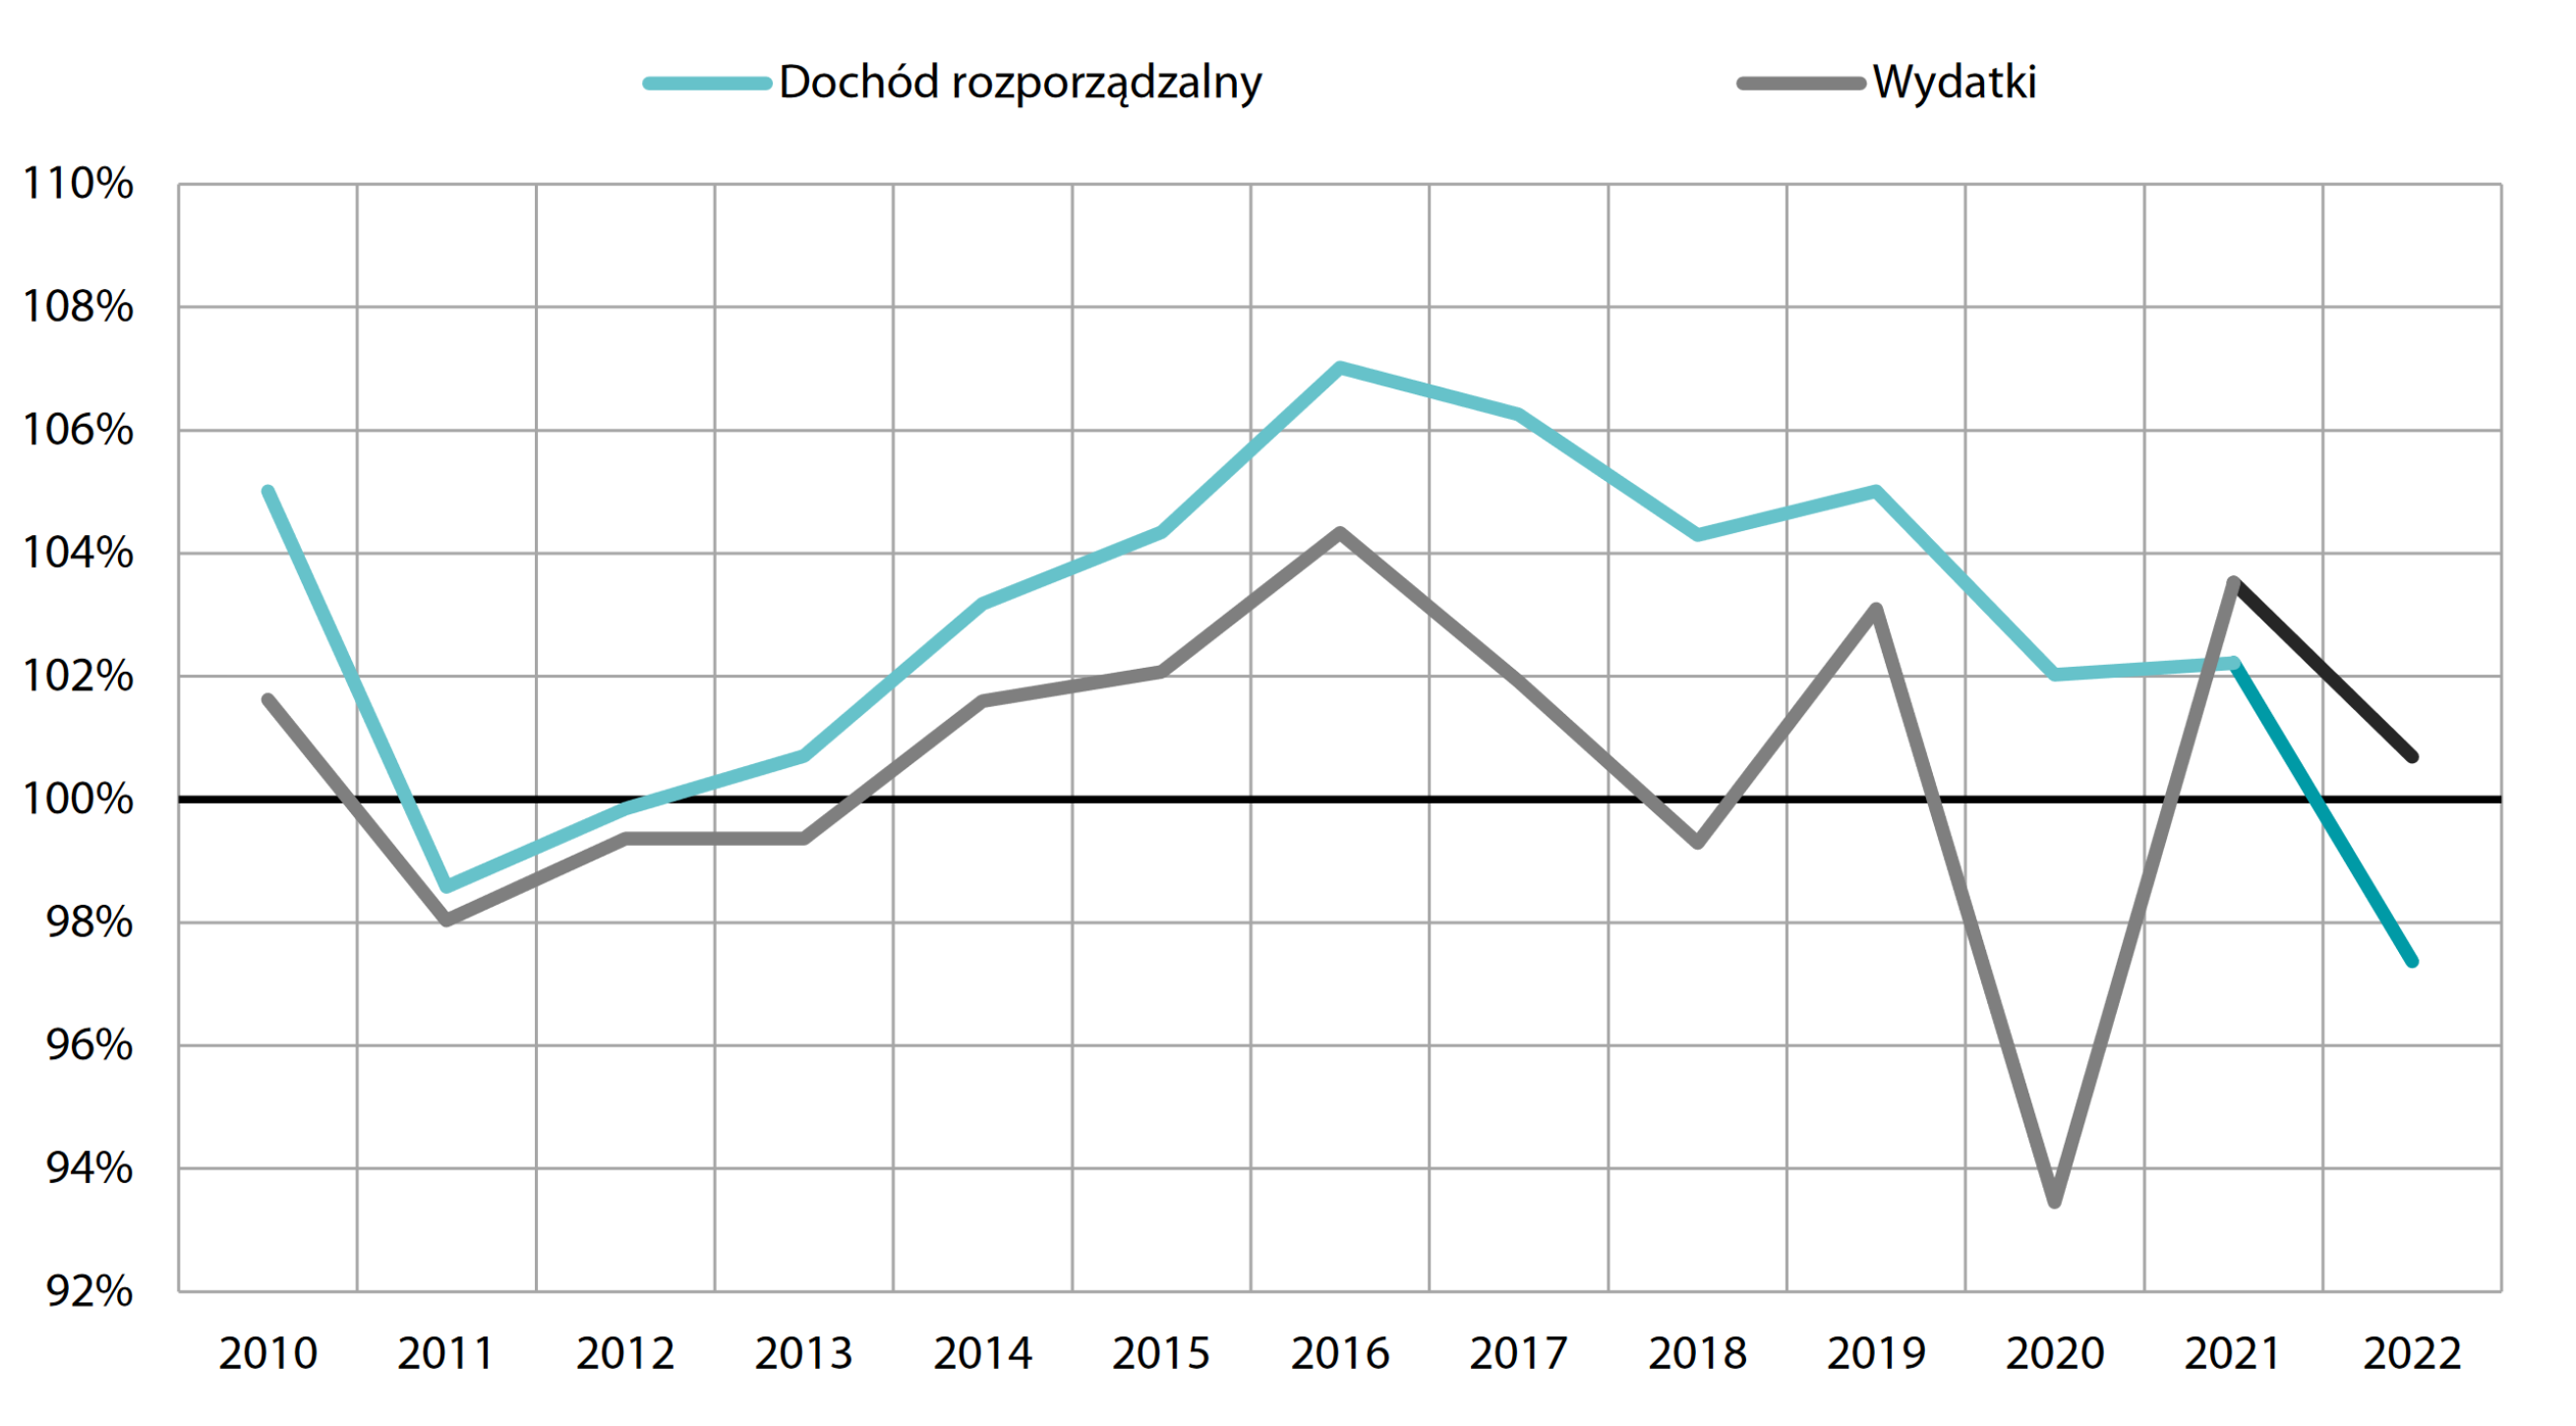
\includegraphics[width=12cm]{figures/GUS_dynamikarealnychdochodowiwydatkow2010-2020.png}
\end{figure}

\begin{figure}[H]           %requires float package
    \caption{300gospodarka.p, Inflacja w Polsce w latach 1996-2023 dane GUS}
    \label{fig:}
    \centering  
    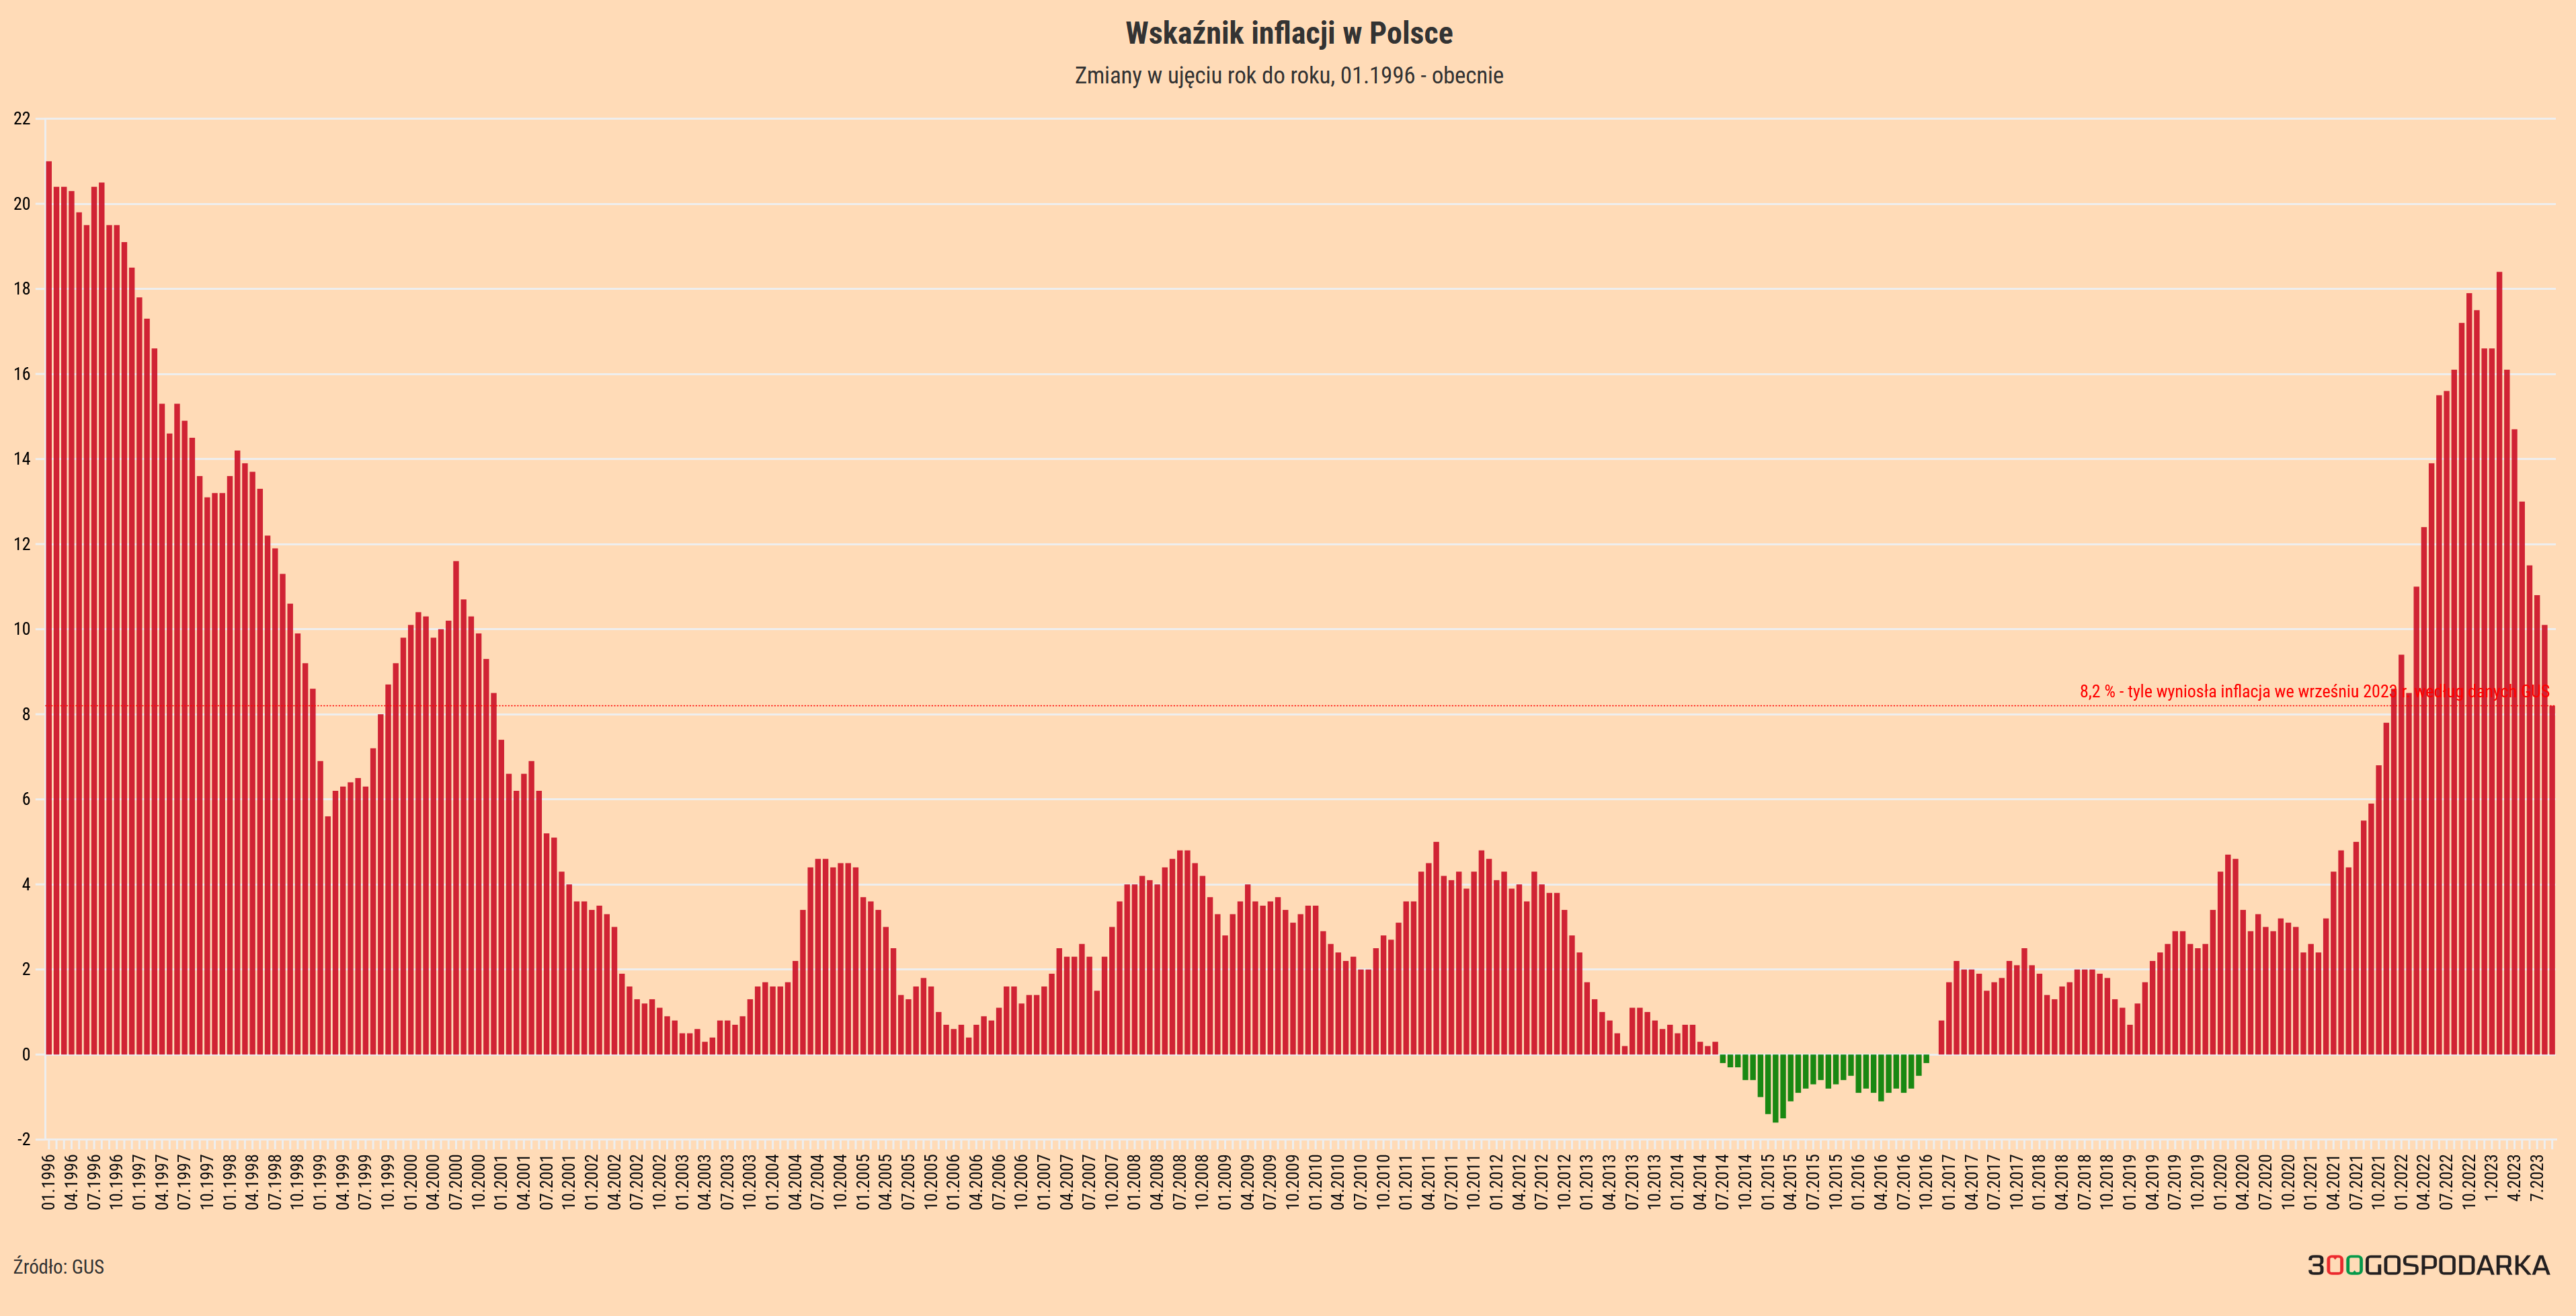
\includegraphics[width=12cm]{figures/300gospodarka-pl_inflacjawpolsce.png}
\end{figure}

{Planowanie domowego budżetu jest podstawowym narzędziem które pomaga utrzymać 
wydatki w ryzach. Skłąda się z dwóch etapów - po pierwsze metody lub narzędzia 
które ułatwią zarządzanie budżetem domowym oraz znajomości podstaw zarządzania 
finansami. Dlatego dla osób rozpoczynających budżetowanie ważne jest 
przedstawienie w możliwie prostej, zwięzłej i przystępnej formie już gotowych 
opracowanych rozwiązań które można zastosować aby świadomie zarządzać sytuacją 
finansową własnego domostwa. W najprostszym wariancie na 
budżet\cite{o24_budzetowanie}\cite{budget}\cite{iwućbudżet}\cite{mintbudget} 
składają się: wpływy czyli dochody ze wszystkich źródeł, zobowiązania czyli 
płatności stałe jak rachunki czy raty kredytów oraz wydatki które są 
zróżnicowane. Skrupulatne zbieranie danych z pewnego okresu pozwala określić 
ogólną sytuację, a w miarę wydłużania zakresu czasu dostępnych danych i 
zwiększania ich precyzja wyłaniają się trendy co umożliwia prognozowanie 
przyszłej sytuacji. Istnieje wiele różnych podejść do tworzenia budżetu - od 
najbardziej ogólnych które skupiają się wyłącznie na określeniu bilansu wydatków
 oraz wpływów, po najbardziej szczegółowe analizy wydatków na poszczególne 
kategorie czy nawet produkty. Każde z podejść ma swoje dobre strony, i w gruncie
 rzeczy wybór odpowiedniego podejścia jest wyłacznie kwestią preferencji.}

\begin{figure}[H]           %requires float package
    \caption{oszczedzaniepieniedzyblog.pl, Najprostszy budżet - przychody}
    \label{fig:}
    \centering  
    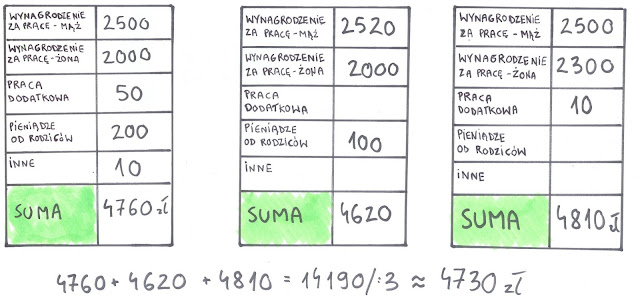
\includegraphics[width=12cm]{figures/oszczedzaniepieniedzyblog-pl_przychody.jpg}
\end{figure}

\begin{figure}[H]           %requires float package
    \caption{oszczedzaniepieniedzyblog.pl, Najprostszy budżet - wydatki}
    \label{fig:}
    \centering  
    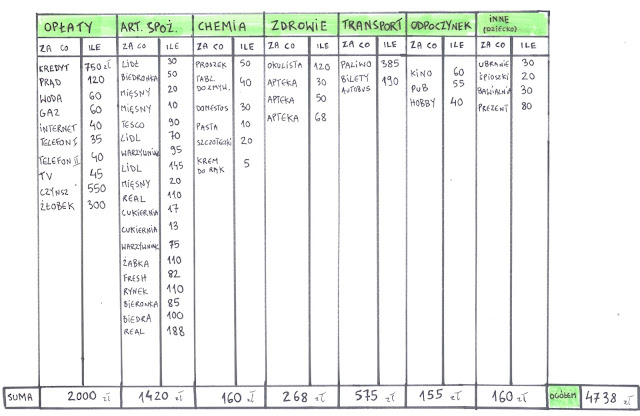
\includegraphics[width=12cm]{figures/oszczedzaniepieniedzyblog-pl_wydatki.jpg}
\end{figure}

{Poza ukazaniem ogólnego obrazu sytuacji finansowej w budżecie uwzględnić można 
cele jak spłata zadłużenia, czy planowany znaczny wydatek, oraz limity 
pomagające ograniczyć wydatki i cele przychodów zwiększające ilość dostępnych 
środków finansowych. W literaturze przedmiotowej opisano także wiele przydatnych
 podejść oraz zasad jak wstępny podział wydatków na podstawie 
priorytetów\cite{najbogatszyczlowiekwbabilonie} czy uwzględnienie oszczędzania 
w formie podejścia najpierw zapłać sobie\cite{najbogatszyczlowiekwbabilonie}
\cite{finansowaforteca} które można zastosować jako strategie zarządzania 
finansami domowymi aby usprawnić budżet lub osiągnąć zamierzony cel. Jednak aby 
zastosować daną strategię trzeba ją najpierw znać, a jak wynika z informacji 
opisanych wcześniej poziom wiedzy z zakresu finansów w Polsce oceniany jest jako
 słaby, dlatego narzędzia do zarządzania finansami powinny, w najprostszej 
formie udostępniać takie informacje w łatwo przystępnej formie, lub przy 
bardziej zaawansowanym podejściu posiadać zabudowane mechanizmy które 
pozwoliłyby użytkownikowi wybrać i zastosować strategię bez potrzeby jej 
dogłębnej znajomości.}

{Z uwagi na tematykę zwyczajowo są to dane bardzo wrażliwe, zatem wymagają 
odpowiednich zabezpieczeń. Idealną opcją dla potencjalnych użytkowników byłoby 
gdyby jako jedyni mieli dostęp do prywatnych danych, oraz mogli sami precyzyjnie
 decydować komu je udostępniają. Przy znaczącej statystycznie liczbie 
użytkowników dane zebrane w aplikacji po odpowiedniej pełnej nieodwracalnej 
anonimizacji i uśrednieniu mogą posłużyć do modelowania wydatków obywateli 
danych regionów, sektorów, segmentów gospodarki lub nawet ogólnie całego 
państwa, co z kolei można wykorzystać zwrotnie w samej aplikacji aby porównać 
model wydatków użytkownika do adekwatnej średniej i zwrócić uwagę na obszary w 
których pozytywnie od niej odstaje działając jako pozytywne wzmocnienie 
dobrego nawyku\cite{pozytywnewzmocnienie}. Tego typu modelowanie jest już 
przeprowadzane przez Główny Urząd Statystyczny, którego raporty publikowane są 
co roku, jest to więc potencjalne źródło najbardziej precyzyjnych danych, które 
mogłoby zostać wykorzystane do porównań.}


% #TODO: Continue from here
% 3.3. Analiza istniejących rozwiązań
% http://siminskionline.pl/seminarium-inzynierskie/struktura-pracy-inzynierskiej/analiza-istniejacych-rozwiazan/
% Pull from documment: https://docs.google.com/document/d/1cYnRqie6xpVnRh8HOuYQZlcuSP_wxj1rPUvHp9FGgDg/edit
\chapter{\customstylechapter{Analiza istniejących rozwiązań}}
{W tym rozdziale przedstawiona zostanie analiza obecnie dostępnych rozwiązań 
opisanego problemu aby określić ich wady i zalety. Jako że budżetowanie jest 
problemem tak starym jak sam wynalazek pieniądza, historycznie powstało wiele 
różnych rozwiązań których celem jest je ułatwić.}

{Podstawową i najprostszą formą budżetu jest zapis na papierze czy chociażby w 
formie księgi zawierającej przychody i wydatki\cite{o24_budzetowanie}. Sposób ten zostanie 
przeanalizowany ponieważ do niedawna była to główna metoda prowadzenia budżetu 
i mimo postępu cyfryzacji i informatyzacji nadal jest szeroko stosowany. Po 
części zastąpiły go rozwiązania komputerowe w formie różnych aplikacji które 
wymagają mniejszych lub większych nakładów pracy od użytkownika. Okazjonalnie 
tego typu zestawienia prowadzone są dziś także w arkuszach kalkulacyjnych.}

{Pierwszą w pełni cyfrową opcją są same witryny kont bankowych\cite{ingbudżet} 
na których klient często może kategoryzować poszczególne transakcje i wyświetlać
 podsumowania oraz określić zakładany budżet. Rozwiązania te są dostępne dla 
każdego klienta danego banku dlatego warto się im przyjrzeć, jako przykład 
posłuży portal banku Santander - centrum24.pl\cite{santandercentrum24} oraz 
narzędzie Budżet w banku ING\cite{ingbudżet}.}

{Na kolejną kategorię rozwiązań składają się aplikacje dedykowane do zarządzania
 budżetem\cite{budget}. Systemy tego typu po wprowadzeniu danych udostępniają 
użytkownikowi cały wachlarz dodatkowych specjalistycznych opcji i narzędzi. 
Omówione zostaną dwa przykłady tego rodzaju aplikacji - Intuit mint\cite{mint} 
oraz Goodbudget\cite{goodbudget}. Na rynku dostępnych jest wiele więcej 
rozwiązań przez co użytkownik ma dowolny wybór, jednak świadomy wybór 
odpowiedniej opcji wymaga od użytkownika dokładnego przeglądu i porównania kilku
 aplikacji.}

\section{\customstylesection{Budżet papierowy lub arkusz kalkulacyjny}}
{Grupa ta obejmuje wiele różnorodnych narzędzi, nierzadko darmowych, lub takich, 
które użytkownik posiada do innych celów. Przykładowe opcje obejmują proste 
rozpiski i podsumowania na katrkach, arkuusze kalkulacyjne jak Microsoft 
Excel\ref{budzetprzykladowyexcel}, Google Sheets, LibreOffice Calc. Największą 
zaletą tych rozwiązań jest prostota dzięki której z tego typu rozwiązania jest 
w stanie skorzystać w zasadzie każdy jednakże odpowiedzialność za manualne 
utrzymanie i dbanie o jakość czy spójność danych spoczywa wyłącznie na 
użytkowniku który jest jednocześnie autorem budżetu. Jedynie w podejściach 
cyfrowych okazjonalnie znaleźć można dodatki służące do automatyzacji części 
funkcji, nie mniej jednak użytkownicy posiadający odpowiedniąwiedzę i 
umiejętności mogą przygotować tego typu mechanizmy osobiście - przykładowo w 
arkuszach kalkulacyjnych jako formuły czy nawet skrypty (np. VBA w Excell) 
jeżeli narzędzie ma taką funkcję. Udostępniają także każde możliwe podejście 
znane użytkownikowi oraz całkowitą wolność wyboru chociażby kategoryzacji. Z 
uwagi na niski prog wejścia w sieci dostępnych jest wiele poradników oraz 
szablonów, choć paradoksalnie jednocześnie jest to wada ponieważ początkującemu 
użytkownikowi trudno się odnaleźć w sporej ilości prezentowanych opcji. Zależnie
 od wykorzystanej technologii (uwzględniając także budżet papierowy) mogą być 
dostępne zarówno lokalnie jak i w przeglądarce.}

{Na uwagę zasługuje również fakt iż podejście takie niejako mimochodem uczy 
użytkownika podstaw finansów i zmusza do refleksji nad swoją sytuacją, co może 
zaowocować wypracowaniem własnych spersonalizowanych systemów dostosowanych pod 
swoje potrzeby i dopasowanych do preferowanych metod pracy lepiej niż pozostałe 
dostępne rozwiązania.}

\begin{figure}[H]           %requires float package
    \caption{https://marciniwuc.com/budzet-domowy-05-wydatki-nieregularne/ Przykładowy budżet w aplikacji Excel}
    \label{budzetprzykladowyexcel}
    \centering  
    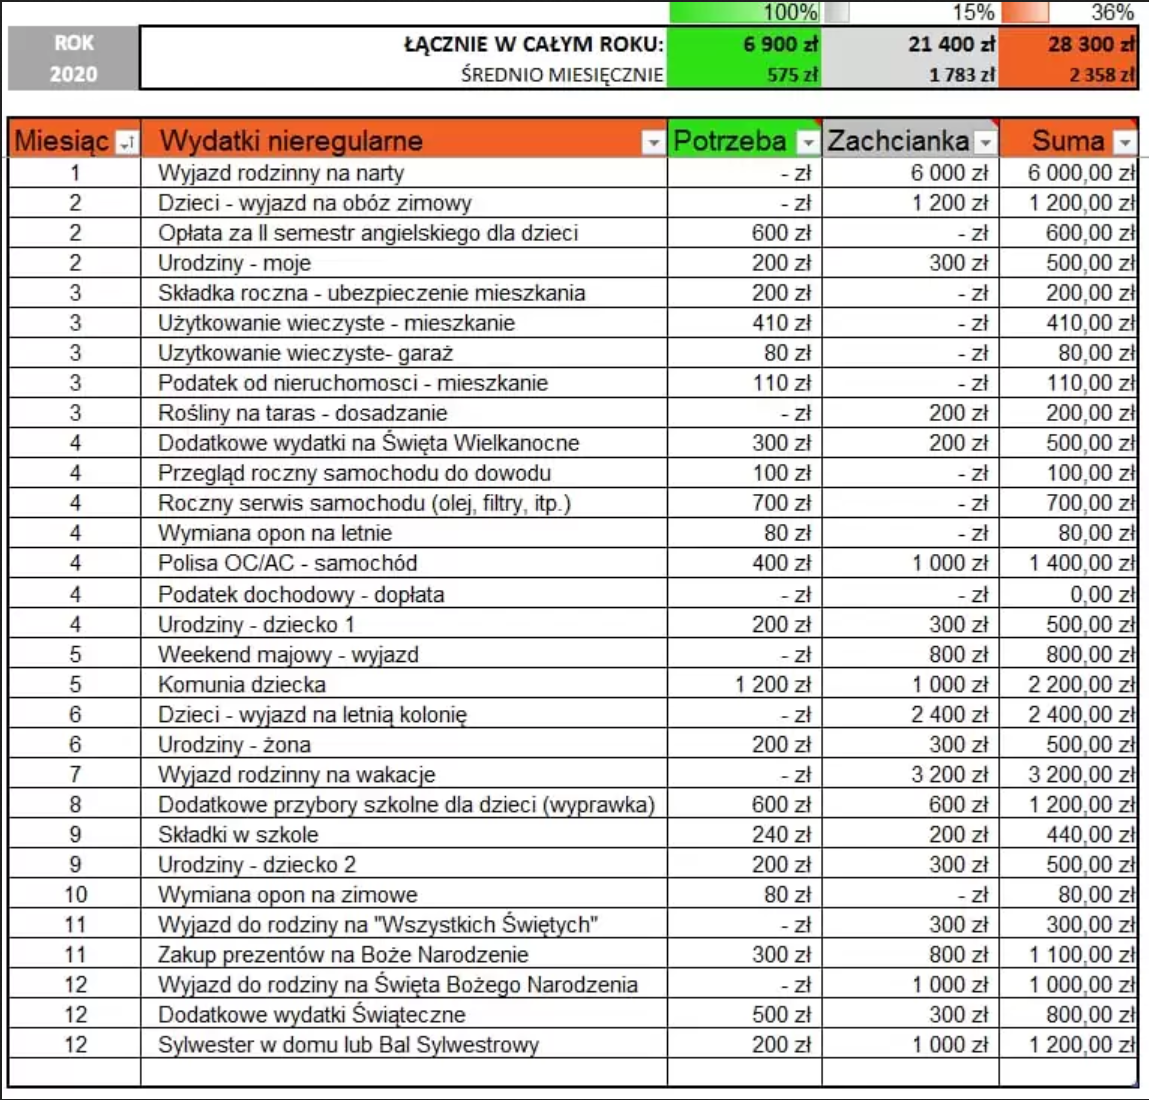
\includegraphics[width=12cm]{figures/marciniwuc.com_Wydatki-nieregularne-plan-roczny.png}
\end{figure}

\begin{figure}[H]           %requires float package
    \caption{https://jakoszczedzacpieniadze.pl/prosty-budzet-domowy Przykładowy budżet na papierze}
    \label{budzetprzykladowypapier}
    \centering  
    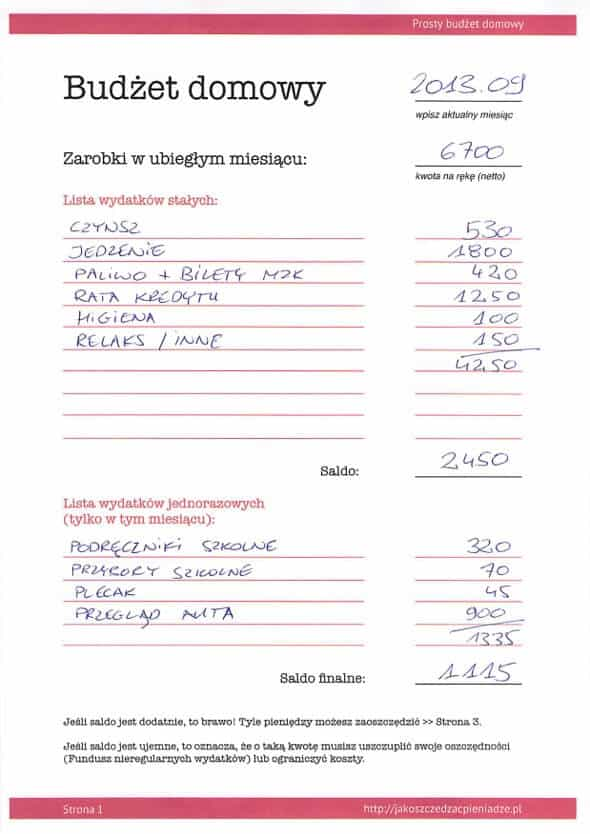
\includegraphics[width=12cm]{figures/jakoszczedzacpieniadze.pl_budzet-domowy-1.jpg}
\end{figure}

\section{\customstylesection{Systemy bankowe - przykład funkcja Budżet w ING Banku Śląskim}}
\section{\customstylesection{Aplikacje dedykowane - Intuit Mint}}
%Worknotes
{darmowa z reklamami lub płatna - ios, android, desktop, ciągłe reklamy, pozwala
 sprawdzić ocenę zdolności kredytowej (TransUnion), popularna 
(25m użytkowników), śledzenie inwestycji, słaba kategoryzacja, powiadomienia i 
przypomnienia (ręcznie), dobre wizualizacje, brak zintegrowanego 
samouczka/instrukcji., Możliwość utworzenia wielu równoczesnych budżetów 
jednocześnie, monitoring subskrybcji, alerty opłat bankowych. Rzekomo dobre 
zabezpieczenia danych.}

\section{\customstylesection{Aplikacje dedykowane - Goodbudget}}
%Worknotes
{mobilna i desktopowa, darmowa (historia rok wstecz) i płatna 
(rozszerzona, historia 7 lat wstecz), system kopertowy (dzielenie przychodów na 
koszyki) z priorytetyzacją i monitoringiem, dobra do współdzielonego budżetu 
(synchronizacja między kontami wielu użytkowników), wskazuje źródła edukacyjne, 
dobre wsparcie i często rozszerzana, ręczne dodawanie wydatków, automatyczna i 
ręczna kategoryzacja, [ręczny?] import danych,}

% [#TODO]:
% 3.3. Analiza istniejących rozwiązań               #TODO: dodaj streszczenie do do 3.1.
% 3.4. Koncepcja własnego rozwiązania               #TODO: dodaj streszczenie do do 3.1.
% 3.5. Projekt ogólny                               #TODO: dodaj streszczenie do do 3.1.
% 3.6. Dokumentacja techniczna                      #TODO: dodaj streszczenie do do 3.1.
% 3.7. Testy i weryfikacja systemu                  #TODO: dodaj streszczenie do do 3.1.
% 3.8. Przykładowy scenariusz wykorzystania systemu #TODO: dodaj streszczenie do do 3.1.
% 3.9. Zakończenie                                  #TODO: dodaj streszczenie do do 3.1.
% 3.13.Ewentualne załączniki


% #TODO: Remove unused sources
% 3.10.Bibliografia
\begin{thebibliography} {books}
    %Books
    \bibitem{najbogatszyczlowiekwbabilonie} George S. Clason, (2021) Najbogatszy człowiek w Babilonie, ISBN: 978-83-67060-04-2
    \bibitem{finansowaforteca} Marcin Iwuć, (2020) Finansowa Forteca, ISBN: 978-83-958468-0-9
    
    %Network resources
    \bibitem{wiki_ekonomia} Wikipedia, Nauki Ekonomiczne \raggedright\url{
        https://pl.wikipedia.org/wiki/Nauki_ekonomiczne}
    \bibitem{zapaśćekonomiczna} Wikipedia, Economic collapse \raggedright\url{
        https://en.wikipedia.org/wiki/Economic_collapse}
    \bibitem{gussytuacjabudzetowa} Główny Urząd Statystyczny, Budżety gospodarstw domowych w 2022 roku \raggedright\url{
        https://stat.gov.pl/obszary-tematyczne/warunki-zycia/dochody-wydatki-i-warunki-zycia-ludnosci/budzety-gospodarstw-domowych-w-2022-roku,9,21.html}
    \bibitem{edukacjafinansowawszkołach} Łukasz Grygiel, Jak wygląda edukacja finansowa dzieci i młodzieży w Polsce? \raggedright\url{
        https://web.archive.org/web/20230529115945/https://lukaszgrygiel.com/edukacja-finansowa-dzieci-i-mlodziezy/}
    \bibitem{edukacjafinansowamlodziezy} Bank Pekao, Raport Banku Pekao: „Dziecięcy świat finansów - jak rynek finansowy odpowiada na potrzeby najmłodszych klientów”. \raggedright\url{
        https://www.pekao.com.pl/o-banku/aktualnosci/d4e423aa-0ba4-4bde-8a0a-7ff3a17a9793/raport-banku-pekao-dzieciecy-swiat-finansow-jak-rynek-finansowy-odpowiada-na-potrzeby-najmodszych-klientow.html}
    \bibitem{portfelpolakawpandemii} Krajowy Rejestr Długów, Portfel statystycznego Polaka w pandemii \raggedright\url{
        https://krd.pl/centrum-prasowe/raporty/2022/portfel-statystycznego-polaka-w-pandemii}
    \bibitem{koszty2010-22} Warsaw Enterprise Institute, [RAPORT] Żegnajcie niskie ceny? Koszty życia i poziom cen w Polsce na tle krajów UE w latach 2010–2022 \raggedright\url{
        https://wei.org.pl/2022/aktualnosci/wiktorwojciechowski/raport-zegnajcie-niskie-ceny-koszty-zycia-i-poziom-cen-w-polsce-na-tle-krajow-ue-w-latach-2010-2022/}
    \bibitem{weiinflacja} Warsaw Enterprise Institute, [RAPORT] Jak inflacja zubaża Polaków? \raggedright\url{
        https://wei.org.pl/2023/publikacje/raporty/mateusz-benedyk/raport-jak-inflacja-zubaza-polakow/}
    \bibitem{o24_budzetowanie} Opcje24, Budzetowanie \raggedright\url{
        https://www.opcje24h.pl/budzetowanie-przewodnik-planowanie-budzetu/}
    \bibitem{iwućbudżet} /marciniwuc.com, Budżet domowy krok po kroku \raggedright\url{
        https://marciniwuc.com/budzet-domowy-krok-po-kroku/}
    \bibitem{ingbudżet} ING Bank Śląski, Jak zapanować nad budżetem domowym? \raggedright\url{
        https://spolecznosc.ing.pl/-/Blog/Jak-zapanowa\%C4\%87-nad-bud\%C5\%BCetem-domowym/ba-p/3968}
    \bibitem{budget} The Balance, Understanding Budgeting \& Personal Finance\raggedright\url{
        https://www.thebalancemoney.com/personal-finance-budget-4802696}
    \bibitem{mintbudget} www.mint.intuit.com, Budgeting 101 \raggedright\url{
        https://mint.intuit.com/blog/category/budgeting/}
    \bibitem{pozytywnewzmocnienie} Simply Scholar, Ltd., Positive Reinforcement: What Is It and How Does It Work? \raggedright\url{
        https://www.simplypsychology.org/positive-reinforcement.html}

    %Evaluated solutions
    \bibitem{santandercentrum24} Santander, Centrum24.pl \raggedright\url{
        https://www.centrum24.pl/}
    \bibitem{mint} Inuit inc., Mint \raggedright\url{
        https://mint.intuit.com/}
    \bibitem{goodbudget} Dayspring Partners, Goodbudget \raggedright\url{
        https://goodbudget.com/}

    %Tools and technologies
    \bibitem{MOSCOW} Product Plan, MOSCOW Prioritetization \raggedright\url{
        https://www.productplan.com/glossary/moscow-prioritization/}
    \bibitem{MatrycaEisenhowera}Praca.pl, Matryca Eisenhowera - czym jest, zasada, prioryteryzacja zadań \raggedright\url{
        https://www.praca.pl/poradniki/rynek-pracy/matryca-eisenhowera-czym-jest,zasada,prioryteryzacja-zadan_pr-2012.html}
    \bibitem{MVP} Wikipedia, Minimal Viable Product \raggedright\url{
        https://en.wikipedia.org/wiki/Minimum_viable_product}
    \bibitem{ISO 8601} NASA.gov, A summary of the international standard date and time notation \raggedright\url{
        https://fits.gsfc.nasa.gov/iso-time.html}
    \bibitem{CSV} Y. Shafranovich, SolidMatrix Technologies, Inc., Common Format and MIME Type for Comma-Separated Values (CSV) Files \raggedright\url{
        https://www.rfc-editor.org/rfc/rfc4180}
    \bibitem{SQLite} sqlite.org, SQLite \raggedright\url{
        https://www.sqlite.org/index.html}
    \bibitem{SQL} wikipedia.org, SQL - Structured Query Language \raggedright\url{
        https://en.wikipedia.org/wiki/SQL}
    \bibitem{Python} python.org, Python \raggedright\url{
        https://www.python.org/}
    \bibitem{JSON} json.org, Introducing JSON \raggedright\url{
        https://www.json.org/json-en.html}
    \bibitem{Python_read-file} pythonspot.com, Python tutorials, How to Read a File in Python \raggedright\url{
        https://pythonspot.com/read-file/}
    \bibitem{Trello} Atlassian, Trello.com \raggedright\url{
        https://trello.com/}
    \bibitem{StarUML} MKLabs Co.,Ltd, StarUML \raggedright\url{
        https://staruml.io/}
    \bibitem{LaTeX} The LaTeX Project \raggedright\url{
        https://www.latex-project.org/}
    \bibitem{VSCode} Microsoft, Visual Studio Code \raggedright\url{
        https://code.visualstudio.com/}
    \bibitem{DataGrid} JetBrains, DataGrid \raggedright\url{
        https://www.jetbrains.com/datagrip/}
    \bibitem{Kanban} Lean Action Plan, Kanban – układ nerwowy sterowania produkcją w koncepcji Lean Manufacturing \raggedright\url{
        https://leanactionplan.pl/kanban/}
    \bibitem{LEAN} Wikipedia, Lean software development \raggedright\url{
        https://pl.wikipedia.org/wiki/Lean_software_development}
    \bibitem{GIT} git-scm.com, git \raggedright\url{
        https://git-scm.com/}
    \bibitem{GitHub} https://github.com/ \raggedright\url{
        https://github.com/}
    \bibitem{Model Przyrostowy} Wikipedia, Model Przyrostowy \raggedright\url{
        https://pl.wikipedia.org/wiki/Model_przyrostowy}
    \bibitem{EdittableTable} YouTube The CS Classroom, PySimpleGUI - Excel-style Editable Table \raggedright\url{
        https://www.youtube.com/watch?v=ETHtvd-_FJg}
    \bibitem{GITBudgeterApp} github.com MarcinNowak94, DatabaseShenanigans \raggedright\url{
        https://github.com/MarcinNowak94/DatabaseShenanigans}
    \bibitem{GITBudgeterDoc} github.com MarcinNowak94, budgeter \raggedright\url{
        https://github.com/MarcinNowak94/budgeter}
    \bibitem{GITRighten} github.com MarcinNowak94, Righten \raggedright\url{
        https://github.com/MarcinNowak94/Righten}
    \bibitem{Bootstrap} getbootstrap.com, Bootstrap \raggedright\url{
        https://getbootstrap.com/}
    \bibitem{Flask} flask.palletsprojects.com, Flask \raggedright\url{
        https://flask.palletsprojects.com/en/3.0.x/}
    \bibitem{WTForms} wtforms.readthedocs.io, WTForms \raggedright\url{
        https://wtforms.readthedocs.io/en/3.1.x/}
    \bibitem{jinja} jinja.palletsprojects.com, Jinja \raggedright\url{
        https://jinja.palletsprojects.com/en/3.1.x/}
    \bibitem{chart.js} www.chartjs.org, Chart.js \raggedright\url{
        https://www.chartjs.org/}        
\end{thebibliography}

% 3.11.Spis rysunków
\listoffigures
% 3.12.Spis tabel
\listoftables
\lstlistoflistings

\end{document}

% Phase 2: Bachelors thesis ----------------------------------------------------
% [DONE]:
% 0. [SELF] Rename projects
% 1. [SELF] Change repository so code and docummentation are in one project
% 2. [SELF] Add Licence
% 3. [Initial review] Change structure to adhere to rules described here:
% http://siminskionline.pl/seminarium-inzynierskie/struktura-pracy-inzynierskiej/
% 3.1. Wstęp <-[sections moved here: Motywacja, cel i plan działania]
% 3.2. Charakterystyka/analiza problemu
% 3.10.Bibliografia
% 3.11.Spis rysunków
% 3.12.Spis tabel


%#TODO: rate this feature